%%%%%%%%%%%%%%%%%%%%%%%%%%%%%%%%%%%%%%%%%%%%%%%%%%%%%%%%%%%%%%%%%%%%%%%%%%%%%%%%%%%%%%%
%%%%%%%%%%%%%%%%%%%%%%%%%%%%%%%%%%%%%%%%%%%%%%%%%%%%%%%%%%%%%%%%%%%%%%%%%%%%%%%%%%%%%%%
% 
% This top part of the document is called the 'preamble'.  Modify it with caution!
%
% The real document starts below where it says 'The main document starts here'.

\documentclass[12pt]{article}

\usepackage{amssymb,amsmath,amsthm}
\usepackage[top=1in, bottom=1in, left=1.25in, right=1.25in]{geometry}
\usepackage{fancyhdr}
\usepackage{graphicx}
\usepackage{enumerate}
\usepackage{verbatim}
\usepackage{listings}
\usepackage{float}

% Comment the following line to use TeX's default font of Computer Modern.
\usepackage{times,txfonts}

\newtheoremstyle{homework}% name of the style to be used
  {18pt}% measure of space to leave above the theorem. E.g.: 3pt
  {12pt}% measure of space to leave below the theorem. E.g.: 3pt
  {}% name of font to use in the body of the theorem
  {}% measure of space to indent
  {\bfseries}% name of head font
  {:}% punctuation between head and body
  {2ex}% space after theorem head; " " = normal interword space
  {}% Manually specify head
\theoremstyle{homework} 

% Set up an Exercise environment and a Solution label.
\newtheorem*{exercisecore}{\@currentlabel}
\newenvironment{exercise}[1]
{\def\@currentlabel{#1}\exercisecore}
{\endexercisecore}

\newcommand{\localhead}[1]{\par\smallskip\noindent\textbf{#1}\nobreak\\}%
\newcommand\solution{\localhead{Solution:}}



% \newcommand{includematlab}[1]{\verbatiminput{#1}}

%%%%%%%%%%%%%%%%%%%%%%%%%%%%%%%%%%%%%%%%%%%%%%%%%%%%%%%%%%%%%%%%%%%%%%%%
%
% Stuff for getting the name/document date/title across the header
\makeatletter
\RequirePackage{fancyhdr}
\pagestyle{fancy}
\fancyfoot[C]{\ifnum \value{page} > 1\relax\thepage\fi}
\fancyhead[L]{\ifx\@doclabel\@empty\else\@doclabel\fi}
\fancyhead[C]{\ifx\@docdate\@empty\else\@docdate\fi}
\fancyhead[R]{\ifx\@docauthor\@empty\else\@docauthor\fi}
\headheight 15pt

\def\doclabel#1{\gdef\@doclabel{#1}}
\doclabel{Use {\tt\textbackslash doclabel\{MY LABEL\}}.}
\def\docdate#1{\gdef\@docdate{#1}}
\docdate{Use {\tt\textbackslash docdate\{MY DATE\}}.}
\def\docauthor#1{\gdef\@docauthor{#1}}
\docauthor{Use {\tt\textbackslash docauthor\{MY NAME\}}.}
\makeatother

%% General formatting parameters
\parindent 0pt
\parskip 12pt plus 1pt

% Shortcuts for blackboard bold number sets (reals, integers, etc.)
\newcommand{\Reals}{\ensuremath{\mathbb R}}
\newcommand{\Nats}{\ensuremath{\mathbb N}}
\newcommand{\Ints}{\ensuremath{\mathbb Z}}
\newcommand{\Rats}{\ensuremath{\mathbb Q}}
\newcommand{\Cplx}{\ensuremath{\mathbb C}}
%% Some equivalents that some people may prefer.
\let\RR\Reals
\let\NN\Nats
\let\II\Ints
\let\CC\Cplx

%%%%%%%%%%%%%%%%%%%%%%%%%%%%%%%%%%%%%%%%%%%%%%%%%%%%%%%%%%%%%%%%%%%%%%%%%%%%%%%%%%%%%%%
%%%%%%%%%%%%%%%%%%%%%%%%%%%%%%%%%%%%%%%%%%%%%%%%%%%%%%%%%%%%%%%%%%%%%%%%%%%%%%%%%%%%%%%
% 
% The main document start here.

% The following commands set up the material that appears in the header.
\doclabel{Math 426: Homework 4}
\docauthor{Stefano Fochesatto}
\docdate{\today}

\newcommand{\vv}{\mathbf{v}}
\begin{document}

\begin{exercise}{Problem 5.1} [Read the bulleted list describing rounding modes on page 116 first.] Write down the IEEE
  double-precision representation for the following decimal numbers,
 
 
 
  \begin{enumerate}
    
    \item 1.5: Using round up,\\

  \solution Using double precision, the number $1.5 = 1.100\times2^0$ is represented by,
  \textbf{Console:}
  \lstinputlisting{5.1.txt}
  Note since $.5$ is a power of two we know that this answer is exact, therefore round down returns the same.



    \item 5.1: Using round to nearest,\\
  
  \solution  Representing $5.1$ in base 2 we get, $101.00\overline{1100}$
  Using double precision, the number $5.1 = 1.0100\overline{0110}\times2^2$ is represented by,
  \textbf{Console:}
  \lstinputlisting{5.1.1.txt}
  Note that with higher precision the next bit would be a $0$ therefore rounding to the nearest will produce the same result. 

    \item -5.1: Using round towards 0, \\
    
  \solution
  Using double precision, the number $-5.1 = -1.0100\overline{0110}\times2^2$ is represented by,
  \textbf{Console:}
  \lstinputlisting{5.1.2.txt}
  Note that rounding to zero a negative number is equivalent to rounding down the corresponding positive, therefore we would produce the same result as the previous problem, for the same reason 

    \item -5.1: Using round to down,\\ 
    
  \solution Using double precision, the number $-5.1 = -1.0100\overline{0110}\times2^2$ is represented by,
  \textbf{Console:}
  \lstinputlisting{5.1.2.txt}
  Rounding to down a negative number is equivalent of rounding up the corresponding positive number, therefore we raise the last digit by adding $(2^-52)_2$. 
  \lstinputlisting{5.1.3.txt}
  
  \end{enumerate}
\end{exercise}


\vspace{.5in}


\begin{exercise}{Problem 5.2} For full credit you should correctly justify via a hand computation how you arrived at this answer. Write down the IEEE double precision representation
  for the decimal number 50.2, round to nearest. \\
  
  \solution First we start by finding the base 2 representation for the number $50.2$. Note that,
  \begin{equation*}
    2^5+2^4+2^1 = 32+16+2 = 50 = (110010)_2.
  \end{equation*}
Now we must find the base 2 representation of $.2 =\frac{1}{5}$. With some binary long division we get,\\

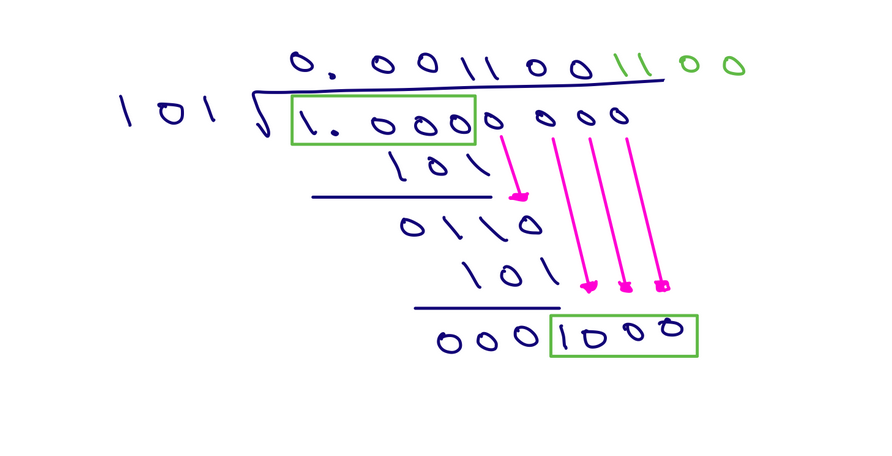
\includegraphics[width = \textwidth]{binarydivision.png}
Therefore the binary representation of $50.2$ is,
\begin{equation*}
  (50.2)_{10} = (110010.00\overline{1100})_2.
\end{equation*}
To get the IEEE double precision representation we need to calculate the sign, mantissa and exponent bits.
The sign bit is easy, since $50.2$ is a positive number we keep the sign bit set to $0$. Since our mantissa has to be of the form,
\begin{equation*}
  1.b_1b_2b_3...b_{52}
\end{equation*}
We know that the decimal will be displaced by 5 digits so therefore the exponent bit will be, 
\begin{equation*}
  (5+1023)_{10} = (1028)_{10} = (10000000100)_2
\end{equation*}
We know what the mantissa bits will be through our binary division, and since we displaced the decimal five digits,
the mantissa will look like the following until it has reached 52 digits (53 if you count the implicit 1),
\begin{equation*}
  (1.1001000\overline{1100})_2
\end{equation*} 
Expanding out to 52 digits and restating the exponents and sign bits we get,
\lstinputlisting{5.1.5.txt}
Following the pattern we know that the next bit will be a $1$ so rounding to the nearest will result in a mantissa of,
\lstinputlisting{5.1.55.txt}
Luckily rounding to nearest was not enough to add another digit and therefore the exponent bits remain unchanged. 

\end{exercise}

\vspace{.5in}





\begin{exercise} {Problem 5.3} What is the gap between 2 and the next larger double-precision number.\\
  \solution 
  From class we know that the gap between $n$ and the next number will be,
  \begin{equation*}
    2^E\epsilon.  
  \end{equation*}
  Where $E$ is the actual exponent for $n$. Since $(2)_{10} = (10)_2$ therefore the actual exponent value is, has to be $1$ in order to get it in the form,
  \begin{equation*}
    1.b_1b_2b_3...b_{52}.
  \end{equation*}
  Substituting $\epsilon = 2^{-52}$ since that is machine epsilon for IEEE double precision, we get that the gap between 2 and the next larger double-precision number is,
  \begin{equation*}
    2^1 2^{-52} = 2^{-51}.
  \end{equation*}
\end{exercise}


\vspace{.5in}


\begin{exercise} {Problem 5.4} What is the gap between 201 and the next larger double precision number.\\
  \solution
  Using the same formula as the last problem, all we need to do is calculate the base 2 representation for 201,
  \begin{equation*}
    201 = 128 + 64 + 8 + 1 = 2^7+2^6+2^3+2^0 = (11001001)_2.
  \end{equation*}
Note that our actual exponent would be $E = 7$, thus 
\begin{equation*}
  2^7 2^{-52} = 2^{-45}.
\end{equation*}
\end{exercise}



\vspace{.5in}





\begin{exercise} {Problem 5.5} How many normalized double-precision numbers are their? Express your answer using powers of 2.\\
\solution
Consider that all double-precision numbers are represented by 1 sign bit, 11 exponent bits and 52 mantissa bits.
Therefore the total representations is calculated by,
\begin{equation*}
  2*2^{11}*2^{52}.
\end{equation*}
However there are two special cases that are not defined as normalized, and those are produced when our exponent bits are all zero, for our two zeroes and subnormal numbers,
and the case where our exponent bits are all ones which is reserved for both infinities and NaNs. Therefore we know that the count of normalized double-precision numbers is,
\begin{equation*}
  2*(2^{11} - 2)*2^{52}.
\end{equation*}

\end{exercise}
\vspace{.5in}

















\begin{exercise} {Problem 5.8} Consider the very limited system in which significands are only of the form,
  \begin{equation*}
    1.b_1b_2b_3,
  \end{equation*}
  and the only exponents are 0,1, and -1. What is the machine precision $\epsilon$ for the system? Assuming that subnormal numbers are not used,
  what is the smallest positive number that can be represented in this system, what is the largest number that can be represented?
  Express you answers in decimal formatting.\\

  \solution
  Calculating machine epsilon by definition,
  \begin{equation*}
    \epsilon = 2^{-3} = .125.
  \end{equation*}
  Calculating the smallest positive number,
  \begin{equation*}
    (1.000)_22^{-1} = .1000 = .5.
  \end{equation*}
  Calculating the largest positive number,
  \begin{equation*}
    (1.111)_22^{1} = 11.11 = 3.75.
  \end{equation*}
\end{exercise}

\vspace{.5in}









\begin{exercise} {Problem 5.9} Consider IEEE double-precision floating-point artithmetic,
  using round to nearest. Let $a, b,$ and $c$ be normalized double-precision floating-point
  numbers, and let $\oplus$, $\ominus$, $\otimes$, and $\oslash$ denote correctly rounded floating-point 
  arithmetic.\\

  \begin{enumerate}
  \item is it necessarily true that $a\oplus b = b\oplus a$? explain why or give a counter example.
  \solution
  Recall the definition of floating point arithmetic,
  \begin{equation*}
    a\oplus b = a + b + error.
  \end{equation*}
  Therefore since regular addition is commutative we get,
  \begin{equation*}
    a\oplus b = a + b + error = b + a + error = b\oplus a.
  \end{equation*}
  \vspace{.25in}


\item Is it necessarily true that  $(a\oplus b )\oplus c = a\oplus (b \oplus c)  $? Explain or give a counterexample\\
\solution
Consider the following Matlab output which uses IEEE double precision with round to nearest,
\textbf{Console:}
\lstinputlisting{5.1.6.txt}
Obviously regular addition is associative, however IEEE addition is not because of the error defined in the definition.

\vspace{.25in}




\item Determine the maximum possible relative error in the computation,
\begin{equation*}
  \dfrac{(a \otimes b)}{c},
\end{equation*}
Assuming that $c \neq 0$. Suppose $c = 0$ that are the possible values that the computation could be assigned. \\
\solution
Recall the definition of relative error,
\begin{equation*}
  e_r = \dfrac{|x -round(x)|}{|x|}.
\end{equation*}
Recall that the maximum $e$ for a round to nearest is,
\begin{equation*}
  e = |x -round(x)| \le \dfrac{2^E\epsilon}{2}.
\end{equation*}
From the inequality,
\begin{align*}
 2^E &\le |x|,\\
\dfrac{1}{|x|} &\le \dfrac{1}{2^E}.
\end{align*}
Thus the maximum relative error is,
\begin{equation*}
  e_r = \dfrac{|x -round(x)|}{|x|} \le \dfrac{\epsilon}{2}.
\end{equation*}
Since the computation,
\begin{equation*}
  \dfrac{(a \otimes b)}{c},
\end{equation*}
is a composition of 2 arithmetic operations we know that the maximum error is $\epsilon$.\\

If we let $c = O$ then there are three cases, if $(a \otimes b)$ is positive then we return positive infinity. If $(a \otimes b)$ is negative then we return negative infinity. If $(a \otimes b)$ is zero we return NaN.  
  \end{enumerate}
\end{exercise}
\vspace{.5in}














\begin{exercise} {Problem 5.15} In the 1991 Gulf War, the Patriot missile defence system failed due to roundoff error. 
  the troubles stemmed fromm a computer that performed the tracking calculations with an internal clock whose integer values in tenths
  of a second were converted to seconds by multiplying by a 24-bit binary approximation of one tenth.\\
  \begin{enumerate}
    \item Convert the binary number in (5.3) into a fraction call it $x$\\
    
    \solution Converting the 24-bit binary approximation of one tenth,
    \begin{equation*}
      x = \dfrac{209715}{2097152}
    \end{equation*}

\item What is the absolute error in $x$,\\

\solution Subtracting,
\begin{equation*}
  |\dfrac{209715}{2097152} -\dfrac{1}{10}| = \dfrac{1}{10485760}.
\end{equation*}


\item What is the time error in seconds after 100 hours of operation,\\

\solution 
\begin{equation*}
  |360000-3600000\frac{209715}{2097152}| \approx 3,240,000.
\end{equation*}

\item  During the 1991 war, a Scud missile traveled at  approximately Mach 5 (3750 mph). Find the distance that a Scud missile would travel during the time error computed in (c)
\solution
\begin{equation*}
  \frac{3240000}{3600}3570 \approx 3,213,000.
\end{equation*}




  \end{enumerate}










\end{exercise}

\end{document}
